% Chapter 2: Background and Related Work
Before explaining the details and implementation of the methodology used in this project, it is essential to provide an overview of the evolution of the inner workings of the Transformer architecture as well as Language Models in general. In addition, we will also discuss relevant compression techniques that have been developed in this context, and how they influenced this work.
Finally, we will also shed some light on the target hardware, whose limitations have been a driving force behind the design choices made in this project.

\section{Early language models}
Before the Transformer architecture, language models were typically based on recurrent neural networks (RNNs). They consists in an extension of the Multi-Layer Perceptron (MLP) in which by integrating cycles, allowing for the network to take into account the previous inputs when making a prediction. For these reason, they can learn long-range dependencies in sequential data, such as text. However, RNNs can be very much prone to the vanishing gradient problem (\ref{rnn_details}), which makes it difficult for them to train in the long run, as during backprogration the contribution of the gradients from earlier layer diminishes exponentially. 

This problem motivated the introduction of the Long Short-Term Memory (LSTM) units, which uses gated cells in order to store more information about the input. In particular, there are three types gate cells:
\begin{itemize}
    \item \textit{Input gate}: controls how much of the new input should be added to the cell state.
    \item \textit{Forget gate}: determines how much of the previous cell state should be retained.
    \item \textit{Output gate}: decides how much of the cell state should be outputted to the next layer.
\end{itemize}
\begin{figure}[!htbp]
    \centering
    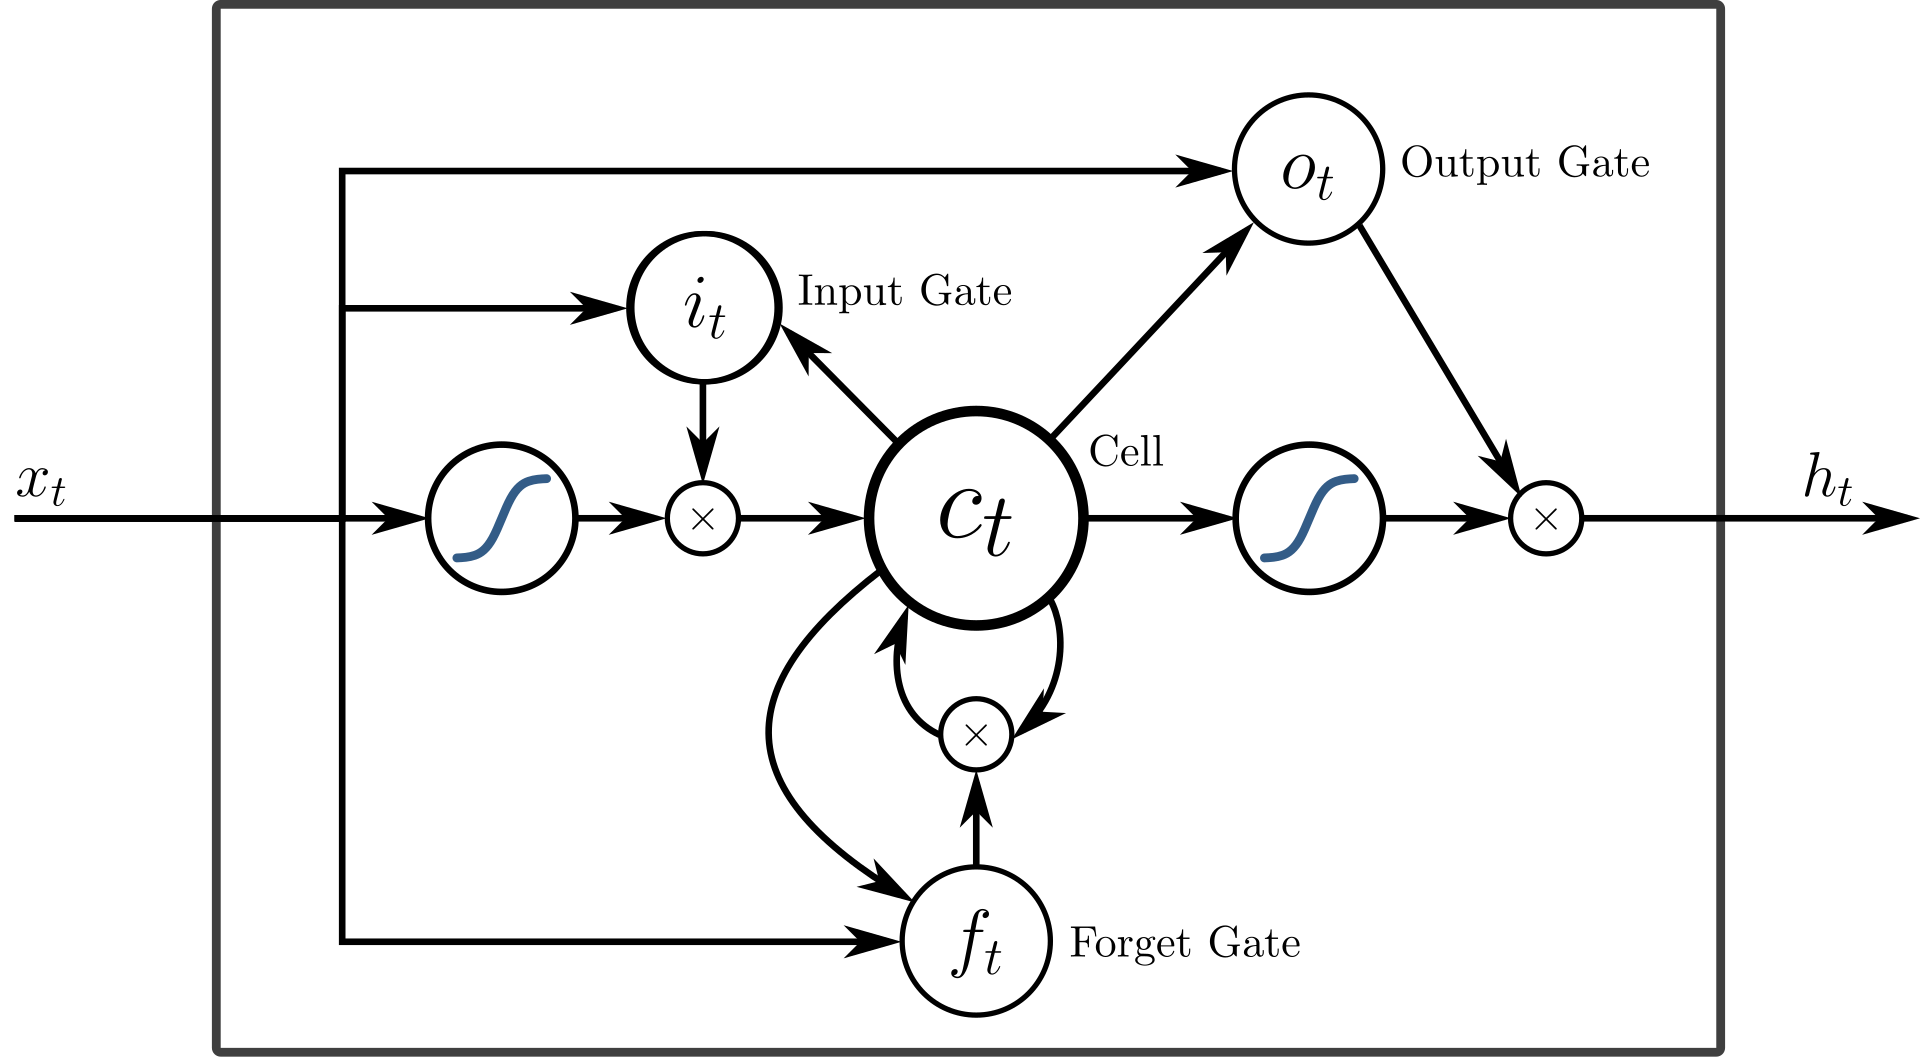
\includegraphics[width=0.7\textwidth]{image.png}
    \caption{A visual representation of the LSTM architecture. The three gates (input, forget, and output) control the flow of information in and out of the cell state, allowing it to retain relevant information over long sequences.}
    \label{fig:your-label}
\end{figure}


\section{The architecture of Transformers}
The Transformer architecture, introduced by Vaswani et al. (2017) [TODO ADD REF HERE], represents a paradigm shift in sequence modeling, moving away from recurrent and convolutional approaches toward a purely attention-based mechanism. This innovation addressed fundamental limitations of previous architectures, particularly the sequential processing bottleneck that hindered parallelization during training.
Attention Mechanism Evolution
The development of attention mechanisms began with Bahdanau et al. (2014), who introduced additive attention to improve neural machine translation by allowing the decoder to focus on relevant parts of the input sequence. This was refined by Luong et al. (2015) with multiplicative attention, which offered computational advantages. However, the breakthrough came with Vaswani et al. (2017), who demonstrated that attention mechanisms alone, without recurrence or convolution, could achieve state-of-the-art results across multiple tasks.
The core innovation lies in the scaled dot-product attention mechanism:
\begin{equation}
\text{Attention}(Q, K, V) = \text{softmax}\left(\frac{QK^T}{\sqrt{d_k}}\right)V
\end{equation}
where Q, K, and V represent queries, keys, and values respectively, and $d_{k}$ is the dimension of the key vectors. This formulation enables efficient computation while capturing long-range dependencies without the sequential constraints of RNNs.

\section{The structure of Large Language Models}

\begin{figure}[htbp]
    \centering
    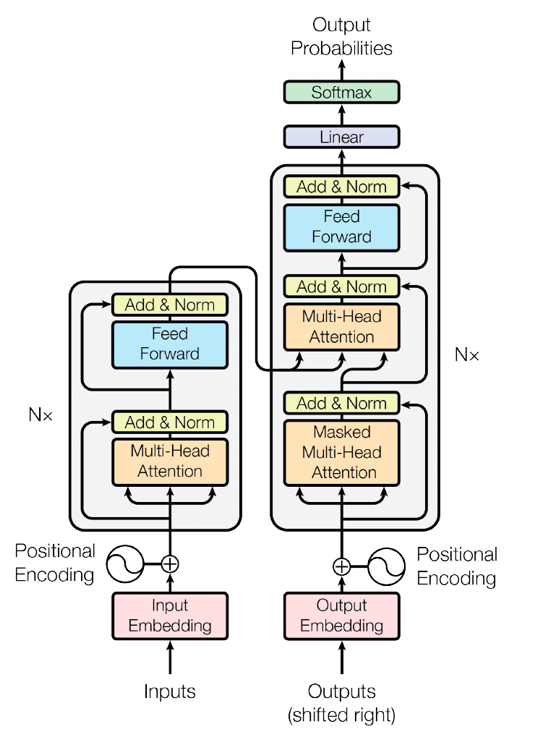
\includegraphics[width=0.45\textwidth]{transformer.png}
    \hfill
    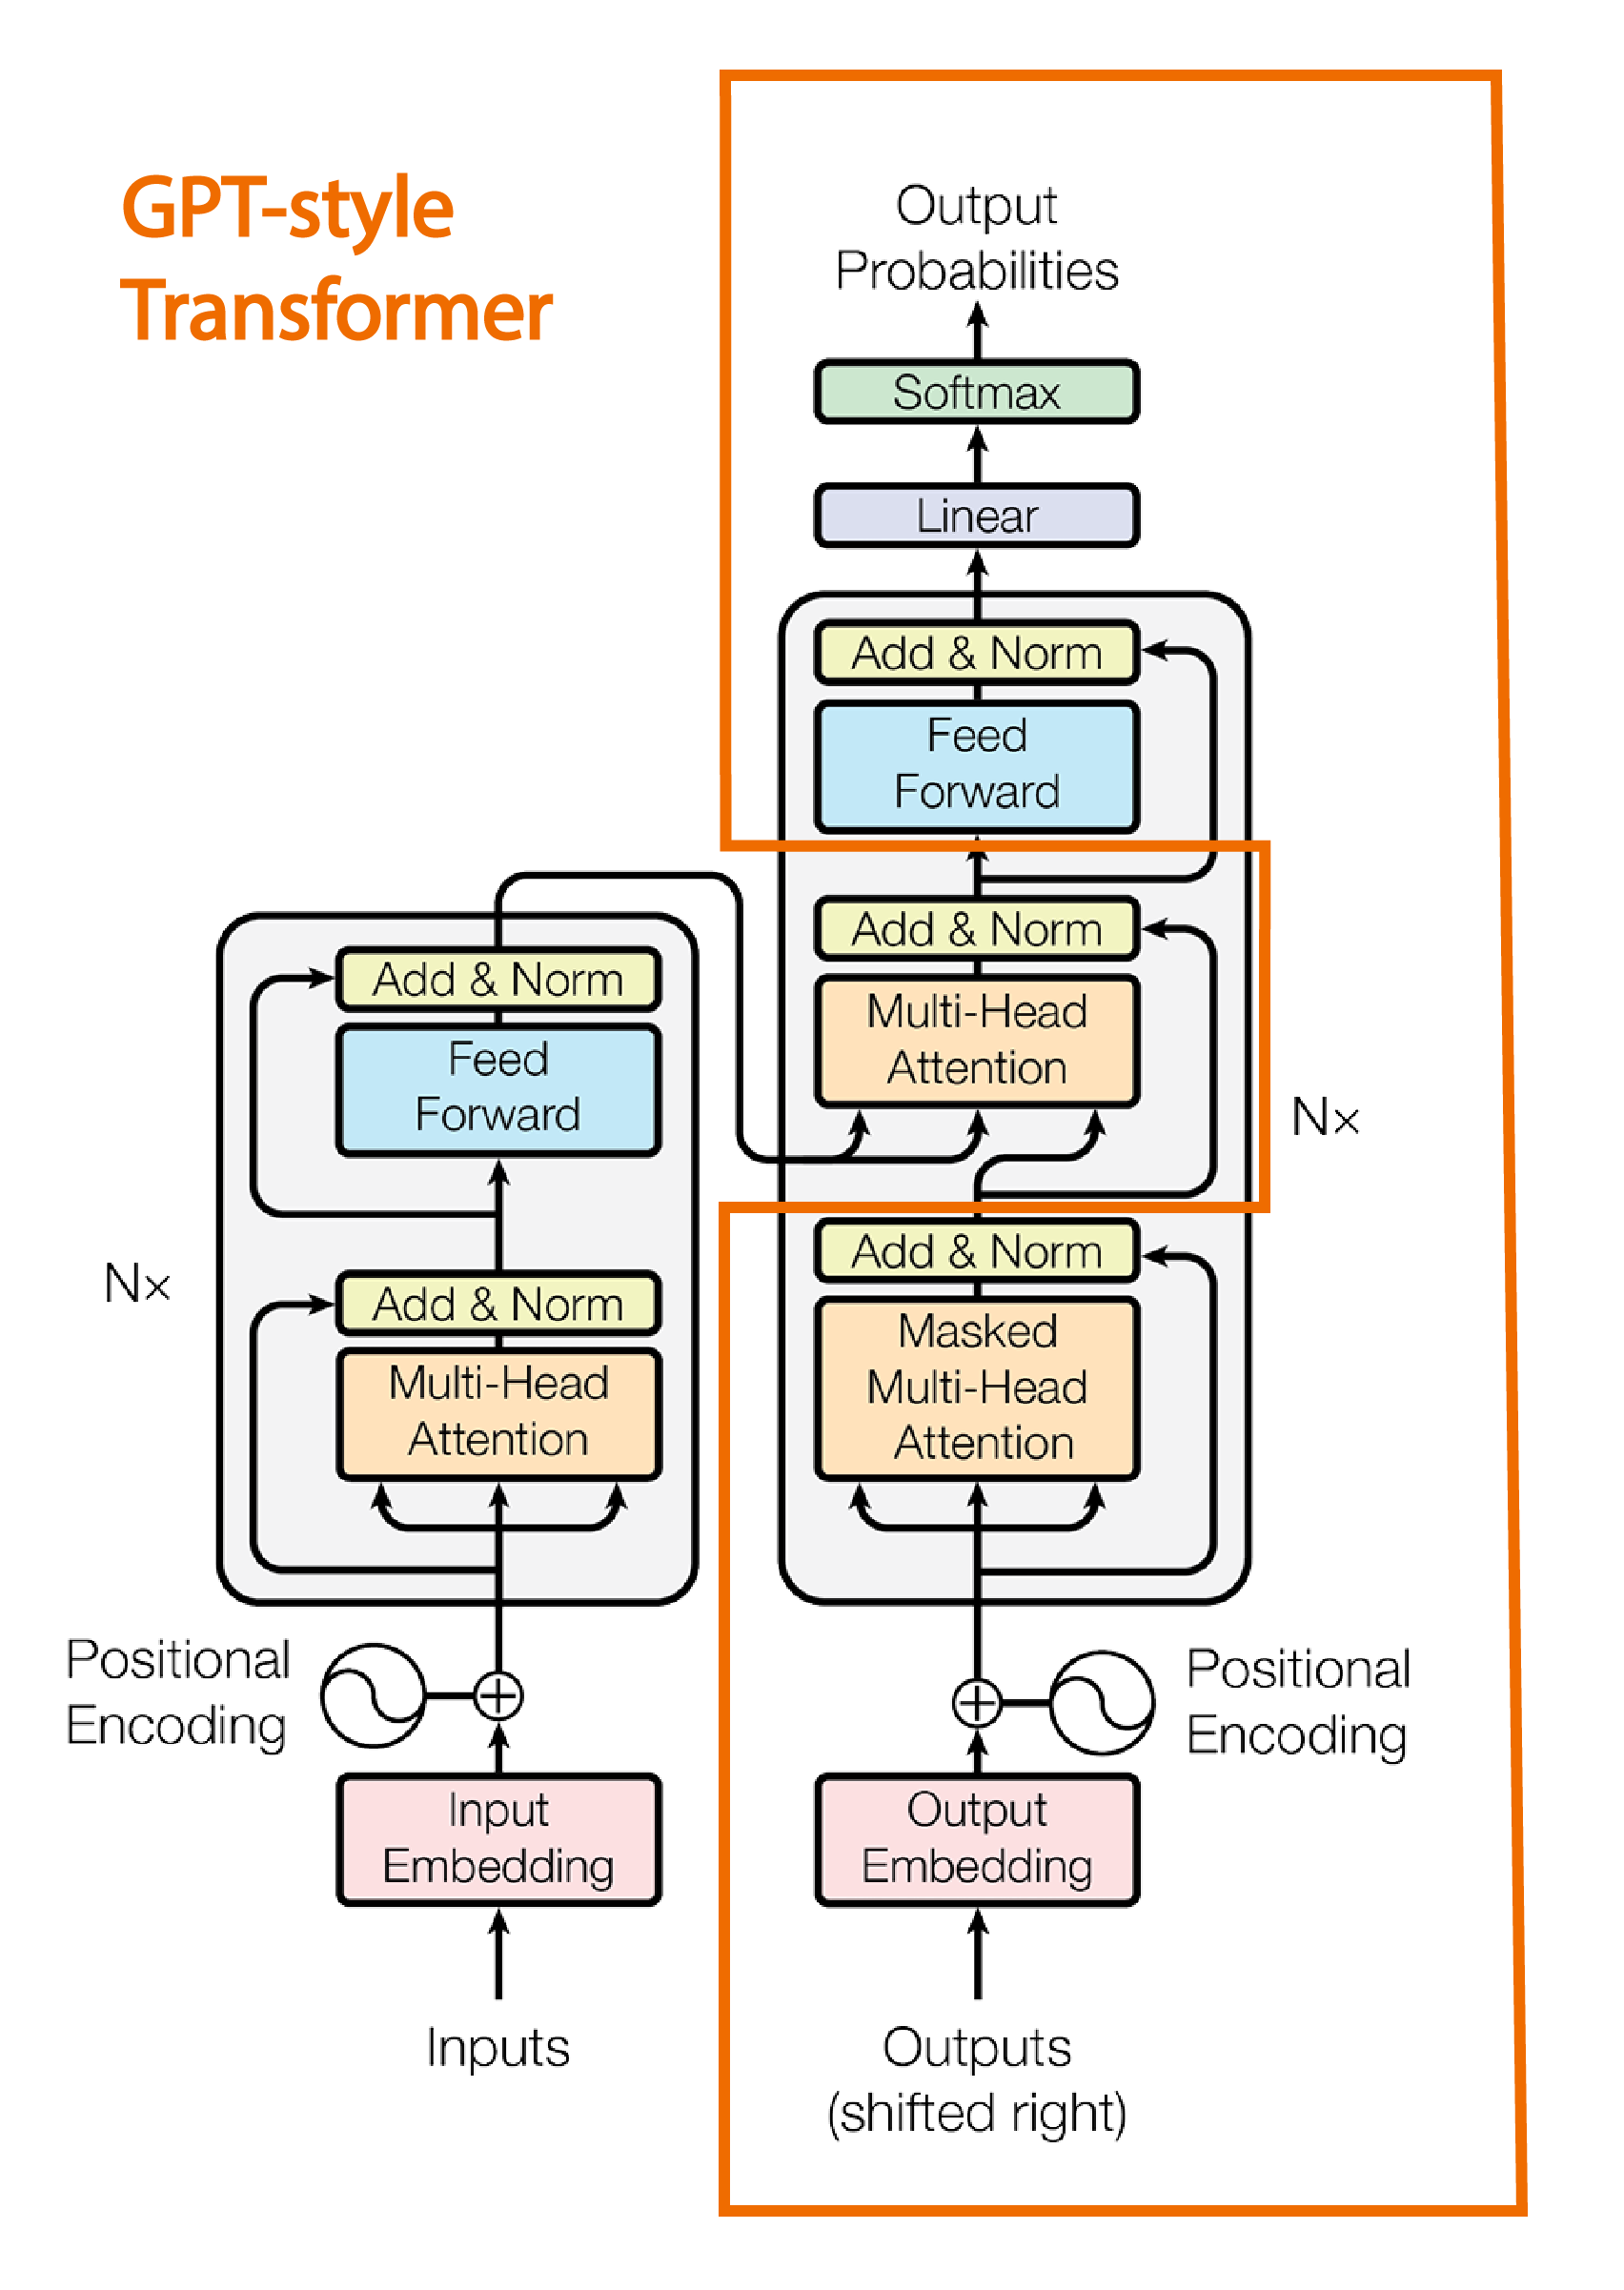
\includegraphics[width=0.45\textwidth]{transformer-gpt.png}
    \caption{On the left, a standard Transformer architecture, which consists of an encoder and a decoder. On the right, we can observe the same architecture, while highlighting the only the layers used by a GPT-style model, which is a decoder-only transformer. The main difference is that the decoder does not attend to the encoder's output, allowing for auto-regressive generation.}
    \label{fig:sidebyside}
\end{figure}

\section{Relevant compression techniques}


